\documentclass[11pt]{article}
\usepackage{dialogue}
% Language setting
\usepackage[turkish]{babel}
\usepackage{pythonhighlight}

\usepackage[a4paper,top=2cm,bottom=2cm,left=2cm,right=2cm,marginparwidth=2cm]{geometry}

% Useful packages
\usepackage{amsmath}
\usepackage{graphicx}
\usepackage[colorlinks=true, allcolors=blue]{hyperref}
\usepackage{verbatim}
\usepackage{fancyhdr} % for header and footer
\usepackage{titlesec}
\usepackage{parskip}

\setlength{\parindent}{0pt}

\titleformat{\subsection}[runin]{\bfseries}{\thesubsection}{1em}{}

\pagestyle{fancy} % activate the custom header/footer

% define the header/footer contents
\lhead{\small{23BLM-4014 Yapay Sinir Ağları Ara Sınav Soru ve Cevap Kağıdı}}
\rhead{\small{Dr. Ulya Bayram}}
\lfoot{}
\rfoot{}

% remove header/footer on first page
\fancypagestyle{firstpage}{
  \lhead{}
  \rhead{}
  \lfoot{}
  \rfoot{\thepage}
}
 

\title{Çanakkale Onsekiz Mart Üniversitesi, Mühendislik Fakültesi, Bilgisayar Mühendisliği Akademik Dönem 2022-2023\\
Ders: BLM-4014 Yapay Sinir Ağları/Bahar Dönemi\\ 
ARA SINAV SORU VE CEVAP KAĞIDI\\
Dersi Veren Öğretim Elemanı: Dr. Öğretim Üyesi Ulya Bayram}
\author{%
\begin{minipage}{\textwidth}
\raggedright
Öğrenci Adı Soyadı: Muhammed Lütfü ÖĞRETİCİ\\ % Adınızı soyadınızı ve öğrenci numaranızı noktaların yerine yazın
Öğrenci No: 190401094
\end{minipage}%
}

\date{14 Nisan 2023}

\begin{document}
\maketitle

\vspace{-.5in}
\section*{Açıklamalar:}
\begin{itemize}
    \item Vizeyi çözüp, üzerinde aynı sorular, sizin cevaplar ve sonuçlar olan versiyonunu bu formatta PDF olarak, Teams üzerinden açtığım assignment kısmına yüklemeniz gerekiyor. Bu bahsi geçen PDF'i oluşturmak için LaTeX kullandıysanız, tex dosyasının da yer aldığı Github linkini de ödevin en başına (aşağı url olarak) eklerseniz bonus 5 Puan! (Tavsiye: Overleaf)
    \item Çözümlerde ya da çözümlerin kontrolünü yapmada internetten faydalanmak, ChatGPT gibi servisleri kullanmak serbest. Fakat, herkesin çözümü kendi emeğinden oluşmak zorunda. Çözümlerinizi, cevaplarınızı aşağıda belirttiğim tarih ve saate kadar kimseyle paylaşmayınız. 
    \item Kopyayı önlemek için Github repository'lerinizin hiçbirini \textbf{14 Nisan 2023, saat 15:00'a kadar halka açık (public) yapmayınız!} (Assignment son yükleme saati 13:00 ama internet bağlantısı sorunları olabilir diye en fazla ekstra 2 saat daha vaktiniz var. \textbf{Fakat 13:00 - 15:00 arası yüklemelerden -5 puan!}
    \item Ek puan almak için sağlayacağınız tüm Github repository'lerini \textbf{en geç 15 Nisan 2023 15:00'da halka açık (public) yapmış olun linklerden puan alabilmek için!}
    \item \textbf{14 Nisan 2023, saat 15:00'dan sonra gönderilen vizeler değerlendirilmeye alınmayacak, vize notu olarak 0 (sıfır) verilecektir!} Son anda internet bağlantısı gibi sebeplerden sıfır almayı önlemek için assignment kısmından ara ara çözümlerinizi yükleyebilirsiniz yedekleme için. Verilen son tarih/saatte (14 Nisan 2023, saat 15:00) sistemdeki en son yüklü PDF geçerli olacak.
    \item Çözümlerin ve kodların size ait ve özgün olup olmadığını kontrol eden bir algoritma kullanılacaktır. Kopya çektiği belirlenen vizeler otomatikman 0 (sıfır) alacaktır. Bu nedenle çözümlerinizi ve kodlarınızı yukarıda sağladığım gün ve saatlere kadar kimseyle paylaşmayınız.
    \item Bu vizeden alınabilecek en yüksek not 100'dür. Toplam aldığınız puan 100'ü geçerse, aldığınız not 100'e sabitlenecektir.
    \item LaTeX kullanarak PDF oluşturanlar öz geçmişlerine LaTeX bildiklerini de eklemeyi unutmasınlar :)
    \item Bu vizedeki soruların çözümleri ve tex dosyası için istediğiniz kadar sayıda Github repository'si oluşturabilirsiniz. Sadece yukarıda belirttiğim tarihlerde (14 Nisan 2023 saat 15:00 ile 15 Nisan 2023 saat 15:00 arasında) public yapmayı/halka açmayı ve Github profilinizi de öz geçmişinize eklemeyi unutmayın :)
    \item Bilgisayarınıza hiçbir program kurmadan, Overleaf, Google Colab, Kaggle gibi ortamlar üzerinden bu vizeyi tamamlamanız mümkün. İyi çalışmalar!!
\end{itemize}

(Ekstra 5 puan)\url{https://github.com/mogretici/YapaySinirAglari/blob/main/ysa.tex}

\newpage
\section{(Toplam 10 Puan) Hopfield Networks:}

\subsection{(2 Puan)} \textbf{ChatGPT’ye size Hopfield Network’ler ile ilgili detaylı bilgi vermesini isteyin. Sorduğunuz soruyu, ChatGPT'nin çıkartığı cevabı aşağı koyun. Bu cevapta anlamadığınız terimleri de ChatGPT’ye sorup, sorduğunuz soruları ve ChatGPT’nin verdiği cevapları da sırayla aşağı koyun.}
\newline
\begin{dialogue}
\speak{SORU} Hopfield Network’ler ile ilgili detaylı bilgi verir misin?
\speak{CHAT-GPT} Tabii, Hopfield Ağı (Hopfield Network), bir tür geri beslemeli yapay sinir ağıdır ve hafıza ve otomatik veri işleme gibi uygulamalar için kullanılır. Adını, John Hopfield adındaki bilim adamından almıştır.

Hopfield Ağı, her biri bir nöronu temsil eden bir dizi bağlantılı nöronun kümesinden oluşur. Her nöron, diğer nöronlarla bağlantılıdır ve her bir bağlantı ağırlık olarak adlandırılan bir sayı ile tanımlanır. Bu ağırlıklar, ağın öğrenme sürecinde belirlenir ve ağın hatırlama ve veri işleme kabiliyetleri üzerinde büyük bir etkiye sahiptir.

Hopfield Ağı, herhangi bir girdi verildiğinde, ağırlıkların güncellenmesi yoluyla girdinin bir temsilini depolar. Daha sonra ağa benzer bir girdi verildiğinde, Hopfield Ağı, öğrenme sürecinde depolanan temsilin benzerliğine göre bir çıktı oluşturur. Bu özellik, Hopfield Ağını desen tanıma ve hatırlama problemleri için ideal hale getirir.

Bununla birlikte, Hopfield Ağı, yalnızca öğrenilen verileri hatırlayabilir ve aynı zamanda bazı dezavantajları da vardır. Örneğin, Hopfield Ağı her zaman global minimuma ulaşmayabilir ve ağırlıkların çoklu öğrenme sürecinde aşırı uyum göstermesi de mümkündür.
\speak{SORU} Geri beslemeli yapay sinir ağı nedir?
\speak{CHAT-GPT} Geri beslemeli yapay sinir ağı (Recurrent Neural Network - RNN), girdilerin geçmiş zaman dilimleriyle de ilişkili olduğu problemlerde kullanılan bir yapay sinir ağı türüdür. Bu ağlar, girdilerin yanı sıra önceki zamandaki çıktıların da ağa geri beslenmesiyle çalışırlar.

Geri beslemeli yapay sinir ağları, birbirine bağlı nöronlardan oluşur. Bu nöronlar, girdileri işlemek için kullanılan geleneksel yapay sinir ağlarındaki nöronlara benzerdir. Ancak geri beslemeli yapay sinir ağlarında, her nöronun ayrıca önceki zamandaki çıktıları da girdi olarak alır ve bu geçmiş zamandaki çıktılar, ağın mevcut çıktısını belirlemede kullanılır.

Bu özellikleri sayesinde geri beslemeli yapay sinir ağları, zaman serileri, dil modelleri, el yazısı tanıma ve konuşma tanıma gibi problemlerde başarılı sonuçlar elde etmek için kullanılır. Örneğin, bir dil modeli, bir cümleyi analiz ederken önceki kelimelerin bağlamını dikkate alarak sonraki kelimeyi tahmin edebilir.

Ancak, geri beslemeli yapay sinir ağları, öğrenme ve eğitim aşamaları daha zorlu ve zaman alıcıdır. Geri besleme döngüleri, ağın eğitimi için ek zorluklar oluşturabilir. Bu nedenle, geri beslemeli yapay sinir ağları, daha basit yapay sinir ağı türlerine göre daha fazla hesaplama kaynağı gerektirir.
\end{dialogue}
\newpage
\subsection{(8 Puan)} \textbf{ChatGPT’nin açıklamalarından ne anladığınızı buraya kendi kelimelerinizle özetleyin. Örneğin ``Hopfield Network nedir? Ne işe yarar? Neden bilmemiz gerekir bunu? Gerçek hayatta kullanılıyor mu?'' gibi. Anlamadığınız kısımlar varsa ve ChatGPT’nin açıklamaları yeterli gelmezse internet dahil farklı kaynaklardan araştırıp, bilgilerin doğruluğunu sorgulamakta serbestsiniz. Konuyu doğru anlayıp anlamamanız puana etki edecektir. Kullandığınız kaynakları da belirtin!}

Hopfield ağları, sinir ağları alanında kullanılan geri beslemeli bir yapay sinir ağı türüdür. Bu ağlar aslında, bir dizi nöronun birbirleriyle bağlantı kurup, etkileşimde bulunduğu modellerdir. Geri besleme döngüsü ve asimetrik bağlantılar olmak üzere iki temel özelliğe sahiptirler. Bu özellikler sayesinde birbirleriyle etkileşime giren nöronlar arasındaki bağlantıların güçlerini değiştirerek öğrenme yapabilirler.

Öğrenme sürecinde ağa bir veri seti gönderilir. Ağ bu veri setini hatırlamak için bağlantılarını güçlendirir. Sonrasında ağa bir girdi verilir ve ağ girdiye en yakın olan veri setini hatırlayarak yeniden oluşturur. Özellikle küçük veri setleri için oldukça etkilidir fakat veri seti büyüyünce bellek boyutu doğrusal olarak arttığından ağın çözümü zorlaşır. 

Bir veri setindeki desenleri tanımak, hatırlamak ve yeniden oluşturmak için yada veriler arasındaki ilişkileri tanımlamak için kullanılabilirler. 

\section{(Toplam 10 Puan) Boltzman Machine:}

\subsection{(2 Puan)} \textbf{ChatGPT’ye size Boltzman Machine ilgili detaylı bilgi vermesini isteyin. Sorduğunuz soruyu, ChatGPT'nin çıkartığı cevabı aşağı koyun. Bu cevapta anlamadığınız terimleri de ChatGPT’ye sorup, sorduğunuz soruları ve ChatGPT’nin verdiği cevapları da sırayla aşağı koyun.}

\begin{dialogue}
\speak{SORU} Boltzman Machine ile ilgili detaylı bilgi verir misin?
\speak{CHAT-GPT} Boltzmann Machine, yapay sinir ağı alanında bir tür oluşturulmuş bir algoritmadır. Bu algoritma, bir tür yapay sinir ağıdır ve öğrenme esnasında, verilerin özelliklerini çıkarır ve bu özellikleri kullanarak veriler arasındaki ilişkileri modeller. Boltzmann Machine, belirli bir veri kümesindeki veri örüntülerini tespit etmek için kullanılabilir. Bu algoritma, her bir veri öğesi arasındaki bağımlılıkları keşfetmek için istatistiksel bir yaklaşım kullanır. Boltzmann Machine, öğrenme sürecinde verilerin dağılımını modellemek için kullanılır ve bu sayede veri kümesindeki örüntüleri çıkarabilir.

Boltzmann Machine, bir dizi nöron ve bağlantı noktalarından oluşur. Bu nöronlar birbirleriyle bağlantılıdır ve birbirlerine sinyal gönderebilirler. Bu sinyaller, ağırlıklandırılmış bir şekilde diğer nöronlara iletilebilir. Bu ağırlıklar, öğrenme sürecinde otomatik olarak belirlenir ve sonuç olarak ağ, belirli bir veri kümesindeki örüntüleri tanımak için kullanılabilir.

Boltzmann Machine, enerji tabanlı bir modeldir. Bu, her bir öğenin bir enerji düzeyine sahip olduğu anlamına gelir. Ağ, enerji fonksiyonunu minimize etmek için optimize edilir. Bu enerji fonksiyonu, ağdaki bağlantıların güçlerine ve her bir nöronun durumuna bağlıdır. Öğrenme süreci, enerji fonksiyonunun minimize edilmesi için gerçekleştirilir. Bu süreç, veri kümesindeki örüntülerin tespit edilmesine yardımcı olur.

Boltzmann Machine, çeşitli uygulamalarda kullanılabilir. Örneğin, resim tanıma, metin sınıflandırma ve konuşma tanıma gibi alanlarda kullanılabilir. Ayrıca, örüntü tanıma ve veri sıkıştırma gibi alanlarda da kullanılabilir.

Sonuç olarak, Boltzmann Machine, yapay sinir ağı alanında kullanılan bir algoritmadır. Bu algoritma, veri kümesindeki örüntüleri tanımlamak ve çıkarmak için kullanılır. Boltzmann Machine, bir enerji fonksiyonu üzerinden çalışır ve veri kümesindeki örüntülerin tespiti için optimize edilir.
\end{dialogue}

\subsection{(8 Puan)} \textbf{ChatGPT’nin açıklamalarından ne anladığınızı buraya kendi kelimelerinizle özetleyin. Örneğin ``Boltzman Machine nedir? Ne işe yarar? Neden bilmemiz gerekir bunu? Gerçek hayatta kullanılıyor mu?'' gibi. Anlamadığınız kısımlar varsa ve ChatGPT’nin açıklamaları yeterli gelmezse internet dahil farklı kaynaklardan araştırıp, bilgilerin doğruluğunu sorgulamakta serbestsiniz. Konuyu doğru anlayıp anlamamanız puana etki edecektir. Kullandığınız kaynakları da belirtin!}

Boltzman Machine özellikle gürültülü, eksik veya belirsiz veri kümelerindeki desenleri tanımak ve tahmin etmek için kullanılan bir enerji tabanlı yapay sinir ağı modelidir. Bir tür denetimsiz öğrenme algoritmasıdır. Giriş verilerinin olasılıksal dağılımlarını öğrenmek için kullanılır. Görünür katman ve gizli katman olmak üzere iki aşamalı yapıya sahiptir. \newline \newline Görünür katman modelin girdisi olarak alınır. Girdi olarak alınan veriler ortak özelliklere göre kümelenip veriler sınıflandırır. Gizli katman ise görünür katmandan gelen verileri işler ve bir çıktı oluşturur.
Çıktıbın başarısı enerji fonksiyonunun değerine göre analiz edilir. Enerji fonksiyonu ne kadar düşük çıkarsa çıktı o kadar başarılıdır.
\newline\newline
Gnünümüzde, resim ve ses tanıma, metin sınıflandırma, örüntü tanıma ve veri sıkıştırma gibi alanlarda kullanılır. 
\newline

\section{(Toplam 10 Puan) Markov Assumption ve Markov Chain:}

\subsection{(2 Puan)} \textbf{ChatGPT’ye size Markov assumption ve Markov Chain ilgili detaylı bilgi vermesini isteyin. Sorduğunuz soruyu, ChatGPT'nin çıkartığı cevabı aşağı koyun. Bu cevapta anlamadığınız terimleri de ChatGPT’ye sorup, sorduğunuz soruları ve ChatGPT’nin verdiği cevapları da sırayla aşağı koyun.}
 
\begin{dialogue}
    \speak{SORU} Markov Chain ilgili detaylı bilgi verir misin?
    \speak{CHAT-GPT}Markov zinciri (Markov Chain), birbirine bağımlı rastgele değişkenlerin (states) bir dizisidir. Bu değişkenler, önceki durumların veya geçmişin değerlerinden bağımsız olarak, yalnızca mevcut durumun değerine bağlıdır. Markov zinciri, bu nedenle Markov özelliği olarak bilinen özelliği paylaşır.

Markov özelliği, bir sistemin gelecekteki durumunun, yalnızca şu anda hangi durumda olduğuna bağlı olduğu anlamına gelir. Bu özellik, birinci dereceden Markov özelliği olarak adlandırılır ve yalnızca bir önceki durumun, mevcut durum üzerinde etkisi olduğu anlamına gelir.

Markov zincirleri, çeşitli uygulama alanlarında kullanılır, özellikle sıralı karar verme, doğal dil işleme, rastgele örüntü tanıma, finansal piyasalar ve genetik algoritmalar gibi alanlarda. Markov zincirleri ayrıca, durumların geçmişine göre gelecekteki olasılıkları hesaplamak için kullanılabilir.

Markov özelliği, bir dizi matematiksel formül ve yöntemle tanımlanabilir. Bu yöntemler arasında, geçiş olasılık matrisi, Markov zincirinin durağan dağılımı ve ergodik teoremi bulunur.

Markov zincirleri, birçok farklı durumda uygulanabilen güçlü bir araçtır. Ancak, Markov zincirleri için önemli bir varsayım olan Markov özelliği, gerçek dünyadaki durumlarda her zaman geçerli değildir. Bu nedenle, Markov zincirleri uygulanırken dikkatli bir şekilde incelenmeli ve özelliğin doğru bir şekilde uygulandığından emin olunmalıdır.
\end{dialogue}
\newpage
\subsection{(8 Puan)} \textbf{ChatGPT’nin açıklamalarından ne anladığınızı buraya kendi kelimelerinizle özetleyin. Örneğin ``Markov assumption ve Markov Chain nedir? Ne işe yarar? Neden bilmemiz gerekir bunu? Gerçek hayatta kullanılıyor mu?'' gibi. Anlamadığınız kısımlar varsa ve ChatGPT’nin açıklamaları yeterli gelmezse internet dahil farklı kaynaklardan araştırıp, bilgilerin doğruluğunu sorgulamakta serbestsiniz. Konuyu doğru anlayıp anlamamanız puana etki edecektir. Kullandığınız kaynakları da belirtin!}

Markov Assumption, sistemin gelecekteki durumunun yalnızca mevcut durumuna bağlı olduğunu varsayar ve geçmişteki durum bilgilerini dikkate almaz. Markov Chain ise Markov Assumption'ın modellenmiş halidir. Durumların zaman içerisindeki gelişimini modellemek için kullanılır. 
\newline \newline Finansal piyasaların modellenmesi, radyoaktif bozunma, trafik akışı analizi, hava durum tahmini gibi bir çok gerçek hayat uygulamasında kullanılırlar. Örneğin bir hisse senedinin fiyatı, hisse senedinin fiyat hareketlerinin bir Markov zinciri olarak modellenmesi yoluyla tahmin edilebilir. Bu modelleme, hisse senedi fiyatlarının gelecekteki fiyat hareketlerini tahmin etmek için kullanılabilir.

\section{(Toplam 20 Puan) Feed Forward:}
 
\begin{itemize}
    \item Forward propagation için, input olarak şu X matrisini verin (tensöre çevirmeyi unutmayın):\\
    $X = \begin{bmatrix}
        1 & 2 & 3\\
        4 & 5 & 6
        \end{bmatrix}$
    Satırlar veriler (sample'lar), kolonlar öznitelikler (feature'lar).
    \item Bir adet hidden layer olsun ve içinde tanh aktivasyon fonksiyonu olsun
    \item Hidden layer'da 50 nöron olsun
    \item Bir adet output layer olsun, tek nöronu olsun ve içinde sigmoid aktivasyon fonksiyonu olsun
\end{itemize}

Tanh fonksiyonu:\\
$f(x) = \frac{exp(x) - exp(-x)}{exp(x) + exp(-x)}$
\vspace{.2in}

Sigmoid fonksiyonu:\\
$f(x) = \frac{1}{1 + exp(-x)}$

\vspace{.2in}
 \textbf{Pytorch kütüphanesi ile, ama kütüphanenin hazır aktivasyon fonksiyonlarını kullanmadan, formülünü verdiğim iki aktivasyon fonksiyonunun kodunu ikinci haftada yaptığımız gibi kendiniz yazarak bu yapay sinir ağını oluşturun ve aşağıdaki üç soruya cevap verin.}
 \newpage
\subsection{(10 Puan)} \textbf{Yukarıdaki yapay sinir ağını çalıştırmadan önce pytorch için Seed değerini 1 olarak set edin, kodu aşağıdaki kod bloğuna ve altına da sonucu yapıştırın:}

% Latex'de kod koyabilirsiniz python formatında. Aşağıdaki örnekleri silip içine kendi kodunuzu koyun
\begin{python}
import torch
import torch.nn as nn

torch.manual_seed(1)
X = torch.tensor([[1, 2, 3], [4, 5, 6]], dtype=torch.float32)
class Net(nn.Module):
    def __init__(self):
        super(Net, self).__init__()
        self.fc1 = nn.Linear(3, 50)
        self.fc2 = nn.Linear(50, 1)
    def tanh(self,x):
      return (torch.exp(x)-torch.exp(-x))/(torch.exp(x)+torch.exp(-x))
    def sigmoid(self,x):
      return 1 / (1 + torch.exp(-x))
    def forward(self, x):
        x = self.fc1(x)
        x = self.tanh(x)
        x= self.fc2(x)
        x = self.sigmoid(x)
        return x
model = Net()
output = model(X)
print(output.data)
\end{python}

tensor([[0.4892],[0.5566]])
\subsection{(5 Puan)} \textbf{Yukarıdaki yapay sinir ağını çalıştırmadan önce Seed değerini öğrenci numaranız olarak değiştirip, kodu aşağıdaki kod bloğuna ve altına da sonucu yapıştırın:}

\begin{python}
import torch
import torch.nn as nn

torch.manual_seed(190401094)
X = torch.tensor([[1, 2, 3], [4, 5, 6]], dtype=torch.float32)
class Net(nn.Module):
    def __init__(self):
        super(Net, self).__init__()
        self.fc1 = nn.Linear(3, 50)
        self.fc2 = nn.Linear(50, 1)
    def tanh(self,x):
      return (torch.exp(x)-torch.exp(-x))/(torch.exp(x)+torch.exp(-x))
    def sigmoid(self,x):
      return 1 / (1 + torch.exp(-x))
    def forward(self, x):
        x = self.fc1(x)
        x = self.tanh(x)
        x= self.fc2(x)
        x = self.sigmoid(x)
        return x
model = Net()
output = model(X)
print(output.data)
\end{python}

tensor([[0.6351],[0.6111]])

\subsection{(5 Puan)} \textbf{Kodlarınızın ve sonuçlarınızın olduğu jupyter notebook'un Github repository'sindeki linkini aşağıdaki url kısmının içine yapıştırın. İlk sayfada belirttiğim gün ve saate kadar halka açık (public) olmasın:}
% size ait Github olmak zorunda, bu vize için ayrı bir github repository'si açıp notebook'u onun içine koyun. Kendine ait olmayıp da arkadaşının notebook'unun linkini paylaşanlar 0 alacak.

\url{https://github.com/mogretici/YapaySinirAglari/blob/main/FeedForward.ipynb}

\section{(Toplam 40 Puan) Multilayer Perceptron (MLP):} 
\textbf{Bu bölümdeki sorularda benim vize ile beraber paylaştığım Prensesi İyileştir (Cure The Princess) Veri Seti parçaları kullanılacak. Hikaye şöyle (soruyu çözmek için hikaye kısmını okumak zorunda değilsiniz):} 

``Bir zamanlar, çok uzaklarda bir ülkede, ağır bir hastalığa yakalanmış bir prenses yaşarmış. Ülkenin kralı ve kraliçesi onu iyileştirmek için ellerinden gelen her şeyi yapmışlar, ancak denedikleri hiçbir çare işe yaramamış.

Yerel bir grup köylü, herhangi bir hastalığı iyileştirmek için gücü olduğu söylenen bir dizi sihirli malzemeden bahsederek kral ve kraliçeye yaklaşmış. Ancak, köylüler kral ile kraliçeyi, bu malzemelerin etkilerinin patlayıcı olabileceği ve son zamanlarda yaşanan kuraklıklar nedeniyle bu malzemelerden sadece birkaçının herhangi bir zamanda bulunabileceği konusunda uyarmışlar. Ayrıca, sadece deneyimli bir simyacı bu özelliklere sahip patlayıcı ve az bulunan malzemelerin belirli bir kombinasyonunun prensesi iyileştireceğini belirleyebilecekmiş.

Kral ve kraliçe kızlarını kurtarmak için umutsuzlar, bu yüzden ülkedeki en iyi simyacıyı bulmak için yola çıkmışlar. Dağları tepeleri aşmışlar ve nihayet "Yapay Sinir Ağları Uzmanı" olarak bilinen yeni bir sihirli sanatın ustası olarak ün yapmış bir simyacı bulmuşlar.

Simyacı önce köylülerin iddialarını ve her bir malzemenin alınan miktarlarını, ayrıca iyileşmeye yol açıp açmadığını incelemiş. Simyacı biliyormuş ki bu prensesi iyileştirmek için tek bir şansı varmış ve bunu doğru yapmak zorundaymış. (Original source: \url{https://www.kaggle.com/datasets/unmoved/cure-the-princess})

(Buradan itibaren ChatGPT ve Dr. Ulya Bayram'a ait hikayenin devamı)

Simyacı, büyülü bileşenlerin farklı kombinasyonlarını analiz etmek ve denemek için günler harcamış. Sonunda birkaç denemenin ardından prensesi iyileştirecek çeşitli karışım kombinasyonları bulmuş ve bunları bir veri setinde toplamış. Daha sonra bu veri setini eğitim, validasyon ve test setleri olarak üç parçaya ayırmış ve bunun üzerinde bir yapay sinir ağı eğiterek kendi yöntemi ile prensesi iyileştirme ihtimalini hesaplamış ve ikna olunca kral ve kraliçeye haber vermiş. Heyecanlı ve umutlu olan kral ve kraliçe, simyacının prensese hazırladığı ilacı vermesine izin vermiş ve ilaç işe yaramış ve prenses hastalığından kurtulmuş.

Kral ve kraliçe, kızlarının hayatını kurtardığı için simyacıya krallıkta kalması ve çalışmalarına devam etmesi için büyük bir araştırma bütçesi ve çok sayıda GPU'su olan bir server vermiş. İyileşen prenses de kendisini iyileştiren yöntemleri öğrenmeye merak salıp, krallıktaki üniversitenin bilgisayar mühendisliği bölümüne girmiş ve mezun olur olmaz da simyacının yanında, onun araştırma grubunda çalışmaya başlamış. Uzun yıllar birlikte krallıktaki insanlara, hayvanlara ve doğaya faydalı olacak yazılımlar geliştirmişler, ve simyacı emekli olduğunda prenses hem araştırma grubunun hem de krallığın lideri olarak hayatına devam etmiş.

Prenses, kendisini iyileştiren veri setini de, gelecekte onların izinden gidecek bilgisayar mühendisi prensler ve prensesler başkalarına faydalı olabilecek yapay sinir ağları oluşturmayı öğrensinler diye halka açmış ve sınavlarda kullanılmasını salık vermiş.''

\textbf{İki hidden layer'lı bir Multilayer Perceptron (MLP) oluşturun beşinci ve altıncı haftalarda yaptığımız gibi. Hazır aktivasyon fonksiyonlarını kullanmak serbest. İlk hidden layer'da 100, ikinci hidden layer'da 50 nöron olsun. Hidden layer'larda ReLU, output layer'da sigmoid aktivasyonu olsun.}

\textbf{Output layer'da kaç nöron olacağını veri setinden bakıp bulacaksınız. Elbette bu veriye uygun Cross Entropy loss yöntemini uygulayacaksınız. Optimizasyon için Stochastic Gradient Descent yeterli. Epoch sayınızı ve learning rate'i validasyon seti üzerinde denemeler yaparak (loss'lara overfit var mı diye bakarak) kendiniz belirleyeceksiniz. Batch size'ı 16 seçebilirsiniz.}

\subsection{(10 Puan)} \textbf{Bu MLP'nin pytorch ile yazılmış class'ının kodunu aşağı kod bloğuna yapıştırın:}

\begin{python}
class MyModel(nn.Module):
    def __init__(self):
        super(MyModel, self).__init__()
        self.fc1 = nn.Linear(len(train_df.columns) - 1, 100) 
        self.fc2 = nn.Linear(100, 50) 
        self.fc3 = nn.Linear(50, 2)
        self.sigmoid = nn.Sigmoid()
    def forward(self, x):
        output = nn.functional.relu(self.fc1(x))
        output = nn.functional.relu(self.fc2(output))
        output = self.fc3(output)
        return self.sigmoid(output)
\end{python}

\subsection{(10 Puan)} \textbf{SEED=öğrenci numaranız set ettikten sonra altıncı haftada yazdığımız gibi training batch'lerinden eğitim loss'ları, validation batch'lerinden validasyon loss değerlerini hesaplayan kodu aşağıdaki kod bloğuna yapıştırın ve çıkan figürü de alta ekleyin.}

\begin{python}
torch.manual_seed(190401094)
def train(model, criterion, optimizer, train_loader, valid_loader, num_epochs):
    for epoch in range(num_epochs):
        model.train()
        train_loss, correct, total = 0.0 , 0 , 0
        for inputs, labels in train_loader:
            inputs = inputs.to(device)
            labels = labels.to(device)
            optimizer.zero_grad()
            outputs = model(inputs)
            loss = criterion(outputs, labels)
            loss.backward()
            optimizer.step()
            train_loss += loss.item()
            _, predicted = outputs.max(1)
            total += labels.size(0)
            correct += predicted.eq(labels).sum().item()
        train_loss /= len(train_loader)
        train_accuracy = 100. * correct / total
        loss_list.append(train_loss)
        model.eval()
        val_loss , val_correct , val_total = 0.0 , 0 , 0
        with torch.no_grad():
            for inputs, labels in valid_loader:
                inputs = inputs.to(device)
                labels = labels.to(device)
                outputs = model(inputs)
                loss = criterion(outputs, labels)
                val_loss += loss.item()
                _, predicted = outputs.max(1)
                val_total += labels.size(0)
                val_correct += predicted.eq(labels).sum().item()
        val_loss /= len(valid_loader)
        val_accuracy = 100. * val_correct / val_total
        val_loss_list.append(val_loss)  
        print(f"Epoch [{epoch+1}/{num_epochs}], Train Loss: {train_loss:.4f}, Train Acc: {train_accuracy:.2f}, Val Loss: {val_loss:.4f}, Val Acc: {val_accuracy:.2f}")
num_epochs = 50
loss_list = []
val_loss_list = []
train(model, criterion, optimizer, train_loader, val_loader, num_epochs)
\end{python}

% Figure aşağıda comment içindeki kısımdaki gibi eklenir.

\begin{figure}[ht!]
    \centering
    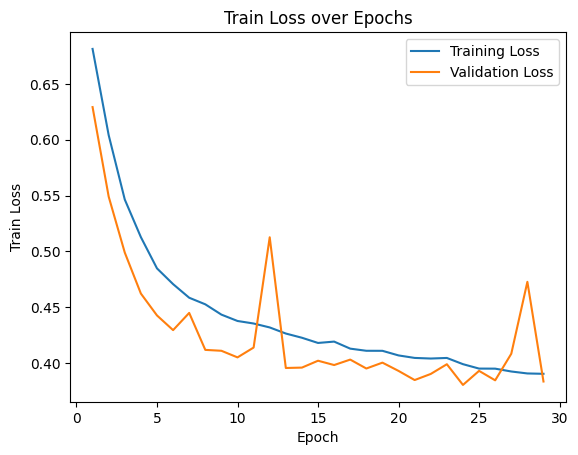
\includegraphics[width=0.75\textwidth]{figure.png}
    \caption{Train Loss Over Epochs }
    \label{fig:figure}
\end{figure}

\newpage
\subsection{(10 Puan)} \textbf{SEED=öğrenci numaranız set ettikten sonra altıncı haftada ödev olarak verdiğim gibi earlystopping'deki en iyi modeli kullanarak, Prensesi İyileştir test setinden accuracy, F1, precision ve recall değerlerini hesaplayan kodu yazın ve sonucu da aşağı yapıştırın. \%80'den fazla başarı bekliyorum test setinden. Daha düşükse başarı oranınız, nerede hata yaptığınızı bulmaya çalışın. \%90'dan fazla başarı almak mümkün (ben denedim).}

\begin{python}
from sklearn.metrics import  accuracy_score, precision_score, f1_score,recall_score
model.eval()
with torch.no_grad():
    true_labels = []
    predicted_labels = []
    for inputs, labels in test_loader:
        inputs = inputs.to(device)
        labels = labels.to(device)
        outputs = model(inputs)
        _, predicted = torch.max(outputs.data, 1)
        true_labels += labels.cpu().numpy().tolist()
        predicted_labels += predicted.cpu().numpy().tolist()
accuracy = accuracy_score(true_labels, predicted_labels)
precision = precision_score(true_labels, predicted_labels, average='weighted', zero_division=1)
recall = recall_score(true_labels, predicted_labels, average='weighted', zero_division=1)
f1 = f1_score(true_labels, predicted_labels, average='weighted', zero_division=1)
print(f"Test Accuracy: {accuracy:.4f}")
print(f"Precision: {precision:.4f}")
print(f"Recall: {recall:.4f}")
print(f"F1 Score: {f1:.4f}")
\end{python}
Test Accuracy: 0.9326
Precision: 0.9357
Recall: 0.9326
F1 Score: 0.9325
\subsection{(5 Puan)} \textbf{Tüm kodların CPU'da çalışması ne kadar sürüyor hesaplayın. Sonra to device yöntemini kullanarak modeli ve verileri GPU'ya atıp kodu bir de böyle çalıştırın ve ne kadar sürdüğünü hesaplayın. Süreleri aşağıdaki tabloya koyun. GPU için Google Colab ya da Kaggle'ı kullanabilirsiniz, iki ortam da her hafta saatlerce GPU hakkı veriyor.}

\begin{table}[ht!]
    \centering
    \caption{Buraya bir açıklama yazın}
    \begin{tabular}{c|c}
        Ortam & Süre (saniye) \\\hline
        CPU & 05.117916 \\
        GPU & 10.261220  \\
    \end{tabular}
    \label{tab:my_table}
\end{table}

\subsection{(3 Puan)} \textbf{Modelin eğitim setine overfit etmesi için elinizden geldiği kadar kodu gereken şekilde değiştirin, validasyon loss'unun açıkça yükselmeye başladığı, training ve validation loss'ları içeren figürü aşağı koyun ve overfit için yaptığınız değişiklikleri aşağı yazın. Overfit, tam bir çanak gibi olmalı ve yükselmeli. Ona göre parametrelerle oynayın.}

Daha fazla epoch eğtimek, veri setinin küçültmek, regülarizasyon kullanmamak yada daha az kullanmak overfitting e neden olan etkenlerdendir. Overfitting yapmak için her epochtan önce validation loss ve training loss değerlerini kontrol edip learning rate i düzenledim. regülarizasyonları kapattım ve epoch sayısını artırdım 

% Figür aşağı
\begin{figure}[ht!]
    \centering
    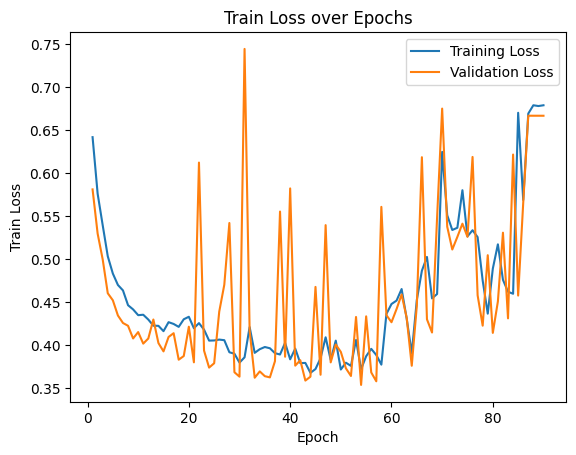
\includegraphics[width=0.5\textwidth]{overfitting.png}
    \caption{Train Loss Over Epochs }
    \label{fig:figure}
\end{figure}

\subsection{(2 Puan)} \textbf{Beşinci soruya ait tüm kodların ve cevapların olduğu jupyter notebook'un Github linkini aşağıdaki url'e koyun.}

\url{https://github.com/mogretici/YapaySinirAglari/blob/main/MultilayerPerceptron.ipynb}\newline
\url{https://github.com/mogretici/YapaySinirAglari/blob/main/Overfitting.ipynb}

\section{(Toplam 10 Puan)} \textbf{Bir önceki sorudaki Prensesi İyileştir problemindeki yapay sinir ağınıza seçtiğiniz herhangi iki farklı regülarizasyon yöntemi ekleyin ve aşağıdaki soruları cevaplayın.} 

\subsection{(2 puan)} \textbf{Kodlarda regülarizasyon eklediğiniz kısımları aşağı koyun:} 

\begin{python}
l1_reg , weight_decay = 0.01 , 0.1 # CoefficientForL1,  CoefficientForL2
    for epoch in range(num_epochs):
        model.train()
        train_loss , correct , total = 0.0 , 0 , 0
        for inputs, labels in train_loader:
            inputs = inputs.to(device)
            labels = labels.to(device)
            optimizer.zero_grad()
            outputs = model(inputs)
            loss = criterion(outputs, labels)
            #StartL1Reg
            # l1_loss = 0
            # for param in model.parameters():
            #     l1_loss += torch.sum(torch.abs(param))
            # loss += l1_reg * l1_loss
            #EndL1Reg
            #StartL2Reg
            l2_reg = 0.0
            for param in model.parameters():
                l2_reg += torch.norm(param)
            loss += weight_decay * l2_reg
            #EndL2Reg
            loss.backward()
            optimizer.step()
            train_loss += loss.item()
            _, predicted = outputs.max(1)
            total += labels.size(0)
            correct += predicted.eq(labels).sum().item()
        train_loss /= len(train_loader)
        train_accuracy = 100. * correct / total
        loss_list.append(train_loss)
        model.eval()
        val_loss , val_correct , val_total = 0.0 , 0 , 0
        with torch.no_grad():
            for inputs, labels in valid_loader:
                inputs = inputs.to(device)
                labels = labels.to(device)
                outputs = model(inputs)
                loss = criterion(outputs, labels)
                #StartL1Reg
                # l1_loss = 0
                # for param in model.parameters():
                #     l1_loss += torch.sum(torch.abs(param))
                # loss += l1_reg * l1_loss
                #EndL1Reg
                #StartL2Reg
                l2_reg = 0.0
                for param in model.parameters():
                    l2_reg += torch.norm(param)
                loss += weight_decay * l2_reg
                # EndL2Reg
                val_loss += loss.item()
                _, predicted = outputs.max(1)
                val_total += labels.size(0)
                val_correct += predicted.eq(labels).sum().item()
        val_loss /= len(valid_loader)
        val_accuracy = 100. * val_correct / val_total
        val_loss_list.append(val_loss)
\end{python}

\subsection{(2 puan)} \textbf{Test setinden yeni accuracy, F1, precision ve recall değerlerini hesaplayıp aşağı koyun:}
\newline
L1 regülarizasyon için değerler: \newline
Test Accuracy: 0.8808
Precision: 0.8846
Recall: 0.8808
F1 Score: 0.8806
\newline
\newline
L2 regülarizasyon için değerler: \newline
Test Accuracy: 0.9093
Precision: 0.9109
Recall: 0.9093
F1 Score: 0.9093

\subsection{(5 puan)} \textbf{Regülarizasyon yöntemi seçimlerinizin sebeplerini ve sonuçlara etkisini yorumlayın:}

 L1 regülarizasyonu, bazı parametreleri tamamen sıfıra eşitlerken, L2 regülarizasyonu tüm parametreleri küçültür ve sıfıra yaklaştırır. Her ikisi de farklı yöntemler kullanarak overfittinge karşı etkili olmayı hedefler. L1 regülarizasyon kullanılarak elde edilen değerler L2 regülarizsyonla elde edilen değerlerden daha yüksek alındı.

\subsection{(1 puan)} \textbf{Sonucun github linkini  aşağıya koyun:}

\url{https://github.com/mogretici/YapaySinirAglari/blob/main/L1andL2Regularizations.ipynb}
\end{document}